\documentclass[aps,prb,twocolumn,superscriptaddress,nofootinbib]{revtex4-2}

\usepackage{graphicx}
\usepackage{amsmath,amssymb}
\usepackage{xcolor}
\usepackage{hyperref}
\hypersetup{colorlinks=true, linkcolor=blue!60!black, citecolor=blue!60!black,
            urlcolor=blue!60!black}
\graphicspath{{../figures/}{figures/}}

% limit the stretch of the glue between floats and text so column balancing
% does not open large gaps below figures
\setlength{\textfloatsep}{12pt plus 2pt minus 3pt}
\setlength{\floatsep}{10pt plus 2pt minus 2pt}
\setlength{\intextsep}{10pt plus 2pt minus 2pt}
\raggedbottom

\newcommand{\I}{\mathcal{I}}

\begin{document}

\title{Demons on a Budget: Adaptive Measurement Placement\\
at the Entanglement Phase Transition}

\author{Rohan Pandey}
\email{rpande.1729@gmail.com}
\affiliation{Independent researcher, Seattle, WA, USA}

\date{\today}

\begin{abstract}
Monitored quantum circuits exhibit a measurement-induced phase transition
between volume-law and area-law entanglement as a function of the
measurement rate $p$. Prior work places measurements at random locations
and treats the rate as the control parameter. We instead fix the
measurement budget and vary the placement process. In brickwork random
Clifford circuits we compare random placement against hand-designed and
reinforcement-learned placement policies at exactly matched budget. We
report three results. First, placement geometry matters more than
placement information: a deterministic contiguous sweep reduces the
half-cut entropy severalfold relative to random placement, while
equal-coverage unstructured placement and a greedy policy with full access
to the quantum state perform far worse than the sweep. Second, the sweep
eliminates the transition rather than shifting it. Tripartite mutual
information crossings recede as $p^\ast \propto 1/L$, the steady-state
entropy saturates at an $L$-independent value close to $0.46/p$, and data
for $L \le 512$ collapse onto the single-scale form $S = p^{-1} f(pL)$
predicted by a ballistic regrowth argument. Third, we account for these
protocols on an exact information ledger. In stabilizer dynamics every
measurement outcome is either deterministic or a fair coin flip, so the
Shannon entropy of the measurement record is exactly countable. The sweep
dominates the resulting entropy-versus-record-cost frontier at every
budget while paying the same cost of approximately one bit per measurement
as random placement. Reinforcement-learned policies trained on the
classical record do not improve on random placement in our experiments,
which we attribute to myopic credit assignment rather than to
expressivity, since the sweep is representable in the policy class. We
conclude that the phase diagram of monitored dynamics is a property of the
placement process, not only of the measurement rate.
\end{abstract}

\maketitle

\section{Introduction}
\label{sec:intro}

Local measurements compete with entangling unitary dynamics. Below a
critical measurement rate $p_c$ a monitored many-body system retains
volume-law entanglement, and above it the state collapses to area
law~\cite{Li2018,Skinner2019,Chan2019}. This measurement-induced phase
transition (MIPT) is a central organizing concept for monitored quantum
matter~\cite{Fisher2023}. Its critical properties have been mapped out for
random Clifford circuits~\cite{Gullans2020,Zabalo2020} and its signatures
have been observed experimentally~\cite{Google2023,Feng2026}.

In nearly all of this literature the measured locations are chosen
uniformly at random. Existing departures from uniform randomness are
static in time. Quasiperiodic measurement sublattices~\cite{Shkolnik2023}
and quenched rate disorder~\cite{Zabalo2023} modify the critical point and
its universality class but preserve the transition. A deterministic
spatial gradient of the rate realizes the transition as coexisting phases
in a single chain~\cite{Li2026space}. Adaptive circuits condition unitary
feedback on measurement outcomes and produce absorbing-state
physics~\cite{Iadecola2023,Sierant2023,ODea2024,Buchhold2022,Piroli2023},
but the measured locations remain random. Closest to our setting,
reinforcement learning has been used to find small sets of projective
measurements that disentangle the output of shallow random circuits; the
structure found there is temporal, a concentration of measurements in late
layers at system sizes of order ten qubits, and the steady-state phase
diagram is not addressed~\cite{Bao2024}. In none of these works is the
spatial placement process itself the designed object.

In this work we take placement as the resource. We fix the expected number
of measurements per layer and ask how much the geometry and the
information content of placement decisions matter, and what they cost. We
model the placing agent as a Maxwell demon that reads part of the
classical measurement record and decides where to look next. In stabilizer
dynamics the demon's ledger can be kept exactly, because each outcome
carries either zero or exactly one bit of Shannon entropy.

The paper is organized as follows. Section~\ref{sec:background} reviews
the concepts and quantities used throughout: entanglement entropy and its
scaling laws, monitored circuits, the stabilizer formalism, the
tripartite mutual information, Landauer's principle, and the policy
optimization methods. Section~\ref{sec:model} defines the model, the
placement policies, and the exact record-entropy ledger.
Section~\ref{sec:geometry} contains the main result: at matched budget, a
deterministic sweeping placement eliminates the volume-law phase, with
finite-size crossings receding as $1/L$ and a single-parameter scaling
collapse across $L = 64$ to $512$, and neither coverage nor state
information reproduces the effect. Section~\ref{sec:ledger} accounts for
all policies on the information ledger. Section~\ref{sec:learned} shows
that policies trained by reinforcement learning fail to discover the
sweep and analyzes why. Section~\ref{sec:discussion} discusses
implications and open questions. Appendices~\ref{app:numerics}
and~\ref{app:learning} give numerical and training details.

\section{Background}
\label{sec:background}

\subsection{Entanglement entropy and its scaling}
For a pure state $|\psi\rangle$ of a chain partitioned into a region $A$
and its complement $B$, the entanglement entropy of $A$ is the von
Neumann entropy of the reduced density matrix,
\begin{equation}
S_A = -\mathrm{Tr}\,(\rho_A \log_2 \rho_A),
\qquad
\rho_A = \mathrm{Tr}_B\, |\psi\rangle\langle\psi|,
\label{eq:vn}
\end{equation}
measured here in bits. Its dependence on the subsystem size
distinguishes phases of dynamics. In a volume-law phase $S_A$ grows
proportionally to the number of sites in $A$, as it does in the
steady state of generic unitary dynamics. In an area-law phase $S_A$
saturates to a constant independent of subsystem size. In one dimension
the boundary of a contiguous region is a pair of points, so area law
means $S_A = O(1)$.

\subsection{Monitored circuits and the MIPT}
A monitored circuit alternates entangling unitary gates with local
projective measurements applied at rate $p$. Each sequence of measurement
outcomes defines a quantum trajectory, and observables are averaged over
trajectories and circuit realizations. Unitary gates spread entanglement
ballistically while measurements remove it locally, and the competition
produces the measurement-induced phase transition: a volume-law phase for
$p < p_c$ and an area-law phase for
$p > p_c$~\cite{Li2018,Skinner2019,Chan2019}. For the brickwork random
Clifford circuit studied here, $p_c \approx 0.16$~\cite{Zabalo2020}.

\subsection{Stabilizer states and Clifford circuits}
A stabilizer state on $n$ qubits is the unique joint $+1$ eigenstate of
an abelian group $S$ of $n$ independent commuting Pauli operators, its
stabilizer group. Clifford gates map Pauli operators to Pauli operators
and therefore map stabilizer states to stabilizer states, which allows
classical simulation in polynomial time~\cite{AaronsonGottesman2004}.
Writing each of the $n$ generators as a binary vector of $X$ and $Z$
components yields the generator matrix $G$ with $n$ rows and $2n$
columns. Entanglement entropies are then exact rank
computations~\cite{Fattal2004}:
\begin{equation}
S_A = \mathrm{rank}_{\mathrm{GF}(2)}\!\left(G|_A\right) - |A|,
\label{eq:rank}
\end{equation}
where $G|_A$ keeps the columns supported on $A$ and arithmetic is
modulo 2. All entropies in this work are computed from
Eq.~\eqref{eq:rank}, with no sampling error beyond the trajectory
ensemble.

\subsection{Tripartite mutual information}
Locating $p_c$ from $S_A$ directly is contaminated by boundary
contributions. The standard diagnostic subtracts them. For contiguous
quarters $A$, $B$, $C$, $D$ of the chain, the tripartite mutual
information is
\begin{equation}
\I_3 = S_A + S_B + S_C - S_{AB} - S_{AC} - S_{BC} + S_{ABC}.
\label{eq:i3}
\end{equation}
Boundary-law terms cancel in this combination, so $\I_3 \to 0$ in the
area-law phase, while in the volume-law phase $\I_3$ is negative and
extensive. Near a conventional critical point $\I_3$ obeys the
finite-size scaling ansatz
\begin{equation}
\I_3(p, L) = \Phi\!\left((p - p_c)\, L^{1/\nu}\right),
\label{eq:fss}
\end{equation}
with $\nu$ the correlation-length exponent, so curves for different $L$
cross at $p = p_c$ and the crossings of successive size pairs converge to
the critical point~\cite{Gullans2020,Zabalo2020}. A transition exists
only if these crossings converge to a finite $p_c$; crossings that recede
toward zero with system size signal the absence of a critical point. The
behavior of the crossings is the key diagnostic in
Sec.~\ref{sec:geometry}.

\subsection{Maxwell's demon and Landauer's principle}
A Maxwell demon is an agent that uses measurement information to reduce
the entropy of a system. The resolution of the associated paradox is
bookkeeping: the demon must record outcomes, and by Landauer's principle
erasing one bit of record costs at least $k_B T \ln 2$ of dissipated
heat~\cite{Landauer1961,Bennett1982}. A consistent account of any
measurement-based protocol therefore weighs the entropy it removes
against the record entropy it writes. Section~\ref{sec:model} shows that
in stabilizer dynamics this record entropy is exactly countable, and
Sec.~\ref{sec:ledger} uses it to compare placement policies.

\subsection{Policy optimization}
A placement policy is a map from an observation to a choice of $k$
measurement sites, and an episode is one circuit run scored by a reward,
here the negative final half-cut entropy. We use two standard
optimizers. The cross-entropy method (CEM) is gradient free: it samples
policy parameters from a Gaussian, keeps the best-scoring fraction, and
refits the Gaussian to the elite set. Proximal policy optimization (PPO)
is a policy-gradient method that ascends the reward while clipping each
update to remain close to the current policy, which stabilizes training.
Both optimize the same objective at matched measurement budget; details
appear in Appendix~\ref{app:learning}.

\section{Model and methods}
\label{sec:model}

\subsection{Monitored Clifford circuits at fixed budget}
We consider a chain of $L$ qubits with periodic boundary conditions. The
chain evolves under brickwork layers of independent uniformly random
two-qubit Clifford gates, interleaved with projective single-site $Z$
measurements. In the standard model each site is measured independently
with probability $p$ per layer. We compare placement processes at matched
budget $pL$ per layer: (i) i.i.d.\ random placement; (ii) the sweep,
which measures a contiguous block that advances around the ring,
\begin{equation}
A_t = \{x_t, x_t + 1, \ldots, x_t + m_t - 1\} \bmod L,
\qquad
x_{t+1} = x_t + m_t,
\label{eq:sweep}
\end{equation}
with $m_t \sim \mathrm{Binomial}(L, p)$ drawn independently each layer,
so that $\mathbb{E}\,|A_t| = pL$ exactly matches the random-placement
budget while the rate $p$ remains continuously tunable; (iii) an
equal-coverage control that visits
every site exactly once per coverage period but in a shuffled order;
(iv) greedy oracle placement at the sites of largest local entanglement,
which uses quantum information unavailable to a physical observer; and
(v) learned policies restricted to classical record information
(Sec.~\ref{sec:learned}). Entanglement entropies are computed exactly
from Eq.~\eqref{eq:rank}, and simulations use
\texttt{stim}~\cite{AaronsonGottesman2004,Gidney2021}. We use circuit
depth $T = 4L$ and locate transitions with the $\I_3$ crossings of
Eq.~\eqref{eq:i3}. Details are given in Appendix~\ref{app:numerics}.

\subsection{An exact information ledger}
The following standard fact makes the demon's ledger exact in stabilizer
dynamics.

\emph{Lemma (bit dichotomy).} Let $|\psi\rangle$ be a stabilizer state on
$n$ qubits with stabilizer group $S$, and let a projective measurement of
$Z_q$ be performed. Either $\pm Z_q \in S$, in which case the outcome is
deterministic and carries zero Shannon entropy, or $Z_q$ anticommutes with
some element of $S$, in which case the two outcomes occur with probability
$1/2$ each and the outcome carries exactly one bit.

\emph{Proof.} If $\pm Z_q \in S$ the state is an eigenstate of $Z_q$ and
the outcome is fixed. Otherwise choose $g \in S$ with $\{g, Z_q\} = 0$.
Then
$\langle \psi | Z_q | \psi \rangle
 = \langle \psi | g^\dagger Z_q g | \psi \rangle
 = - \langle \psi | Z_q | \psi \rangle = 0$,
so the outcomes are unbiased~\cite{AaronsonGottesman2004,Fattal2004}.
\hfill$\square$

The Shannon entropy of the measurement record in a trajectory therefore
equals the number of nondeterministic outcomes, which we count exactly
during simulation via a pre-measurement determinism check. This number is
the minimum memory a demon implementing the policy must write. By
Landauer's principle, $k_B T \ln 2$ times this number bounds the heat cost
of erasing the record~\cite{Landauer1961,Bennett1982}.

\begin{figure*}
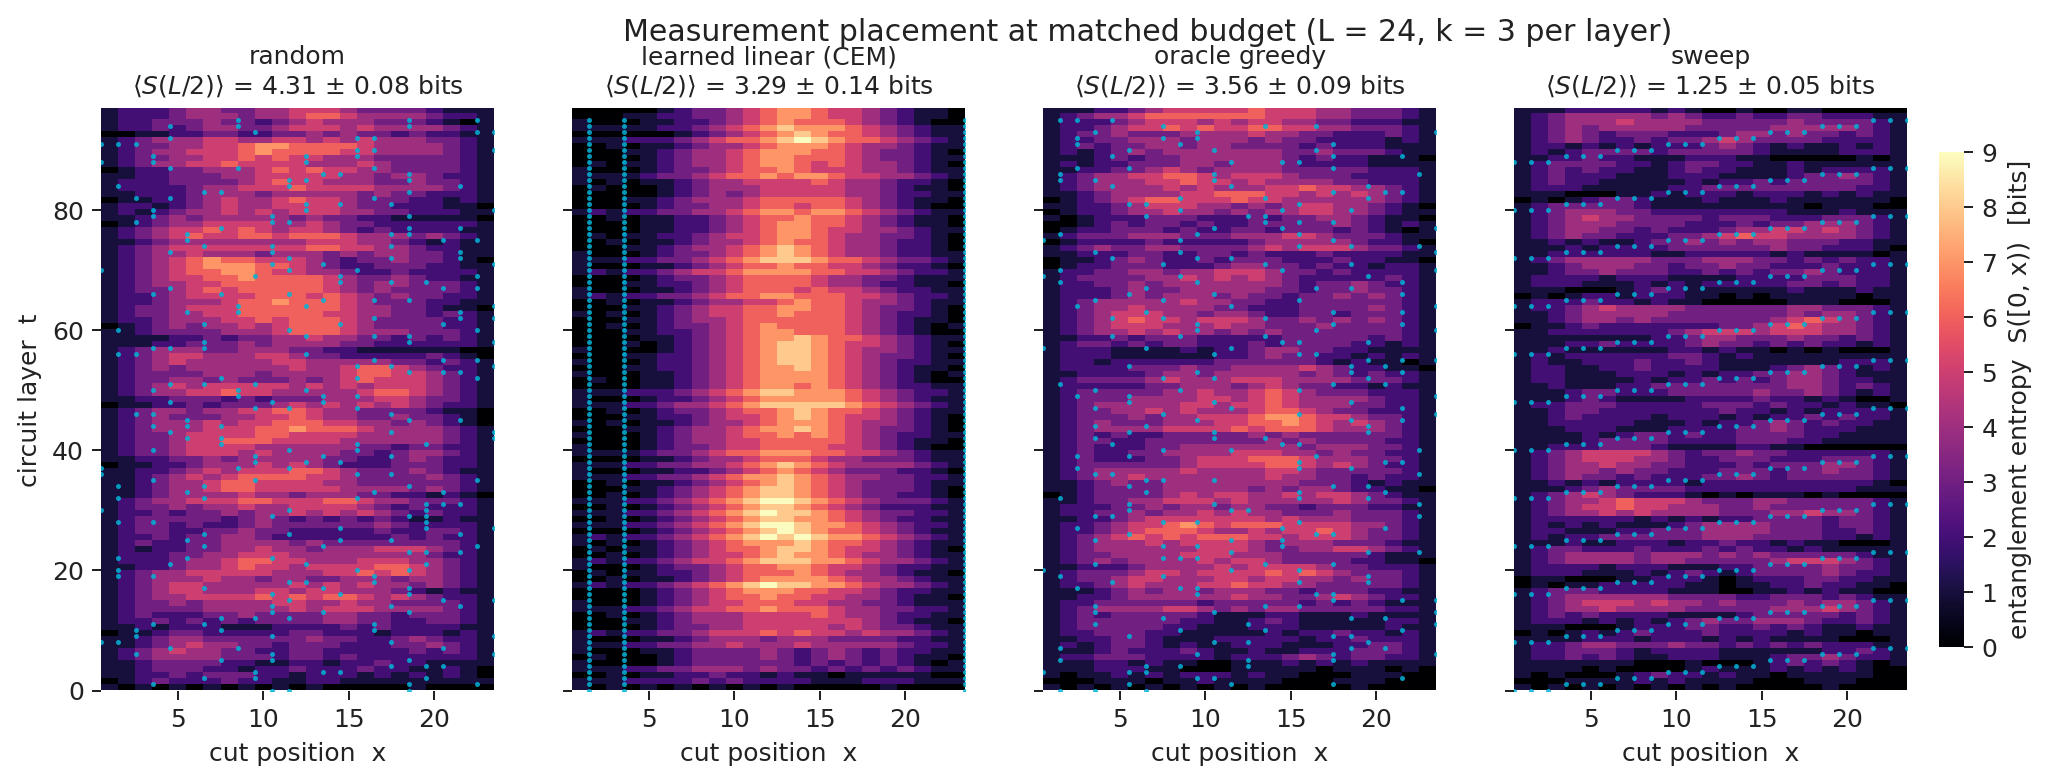
\includegraphics[width=\textwidth]{fig4_spacetime.png}
\caption{Entanglement profile $S([0,x))$ as a function of cut position $x$
and layer $t$ under four placement policies at matched budget ($L{=}24$,
$k{=}3$ per layer). Dots mark measurement events. Titles give
ensemble-mean final entropies. The learned linear policy pins measurements
at fixed sites and fences entanglement into a protected region; the sweep
produces the lowest entropy of all policies studied.}
\label{fig:spacetime}
\end{figure*}

\section{Placement geometry eliminates the transition}
\label{sec:geometry}

\begin{figure}
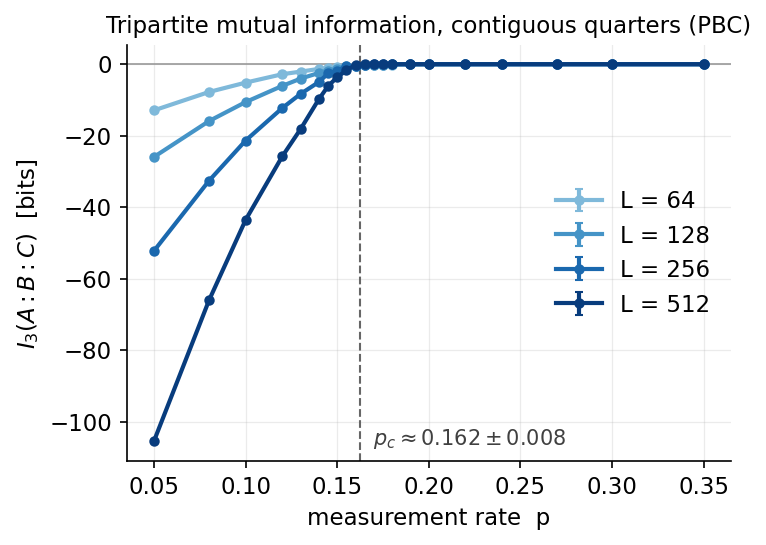
\includegraphics[width=\columnwidth]{fig2_I3_crossing.png}
\caption{Random placement baseline. $\I_3$ crossings for $L = 64$--$512$
give $p_c = 0.162(8)$.}
\label{fig:baseline}
\end{figure}

\begin{figure}
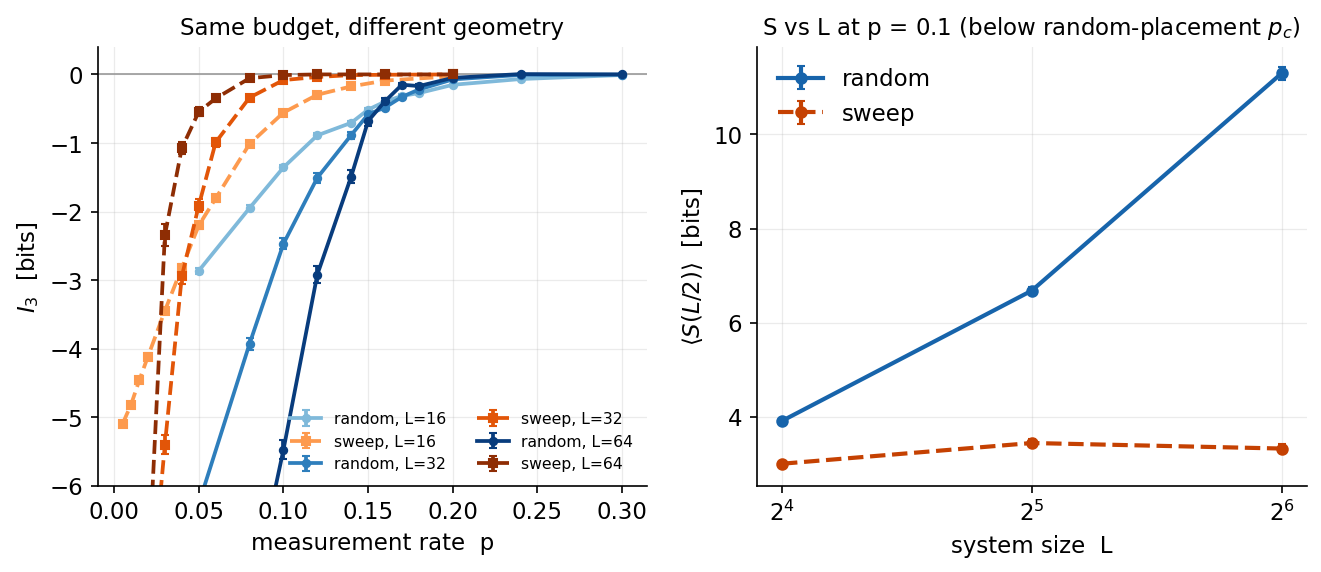
\includegraphics[width=\columnwidth]{fig5_phase_shift.png}
\caption{Identical budget, different geometry. Sweep-placement $\I_3$
curves (dashed) approach zero far below the random-placement transition
(solid), and $S$ versus $L$ at fixed $p = 0.1 < p_c$ is flat under the
sweep.}
\label{fig:phaseshift}
\end{figure}

\begin{figure}
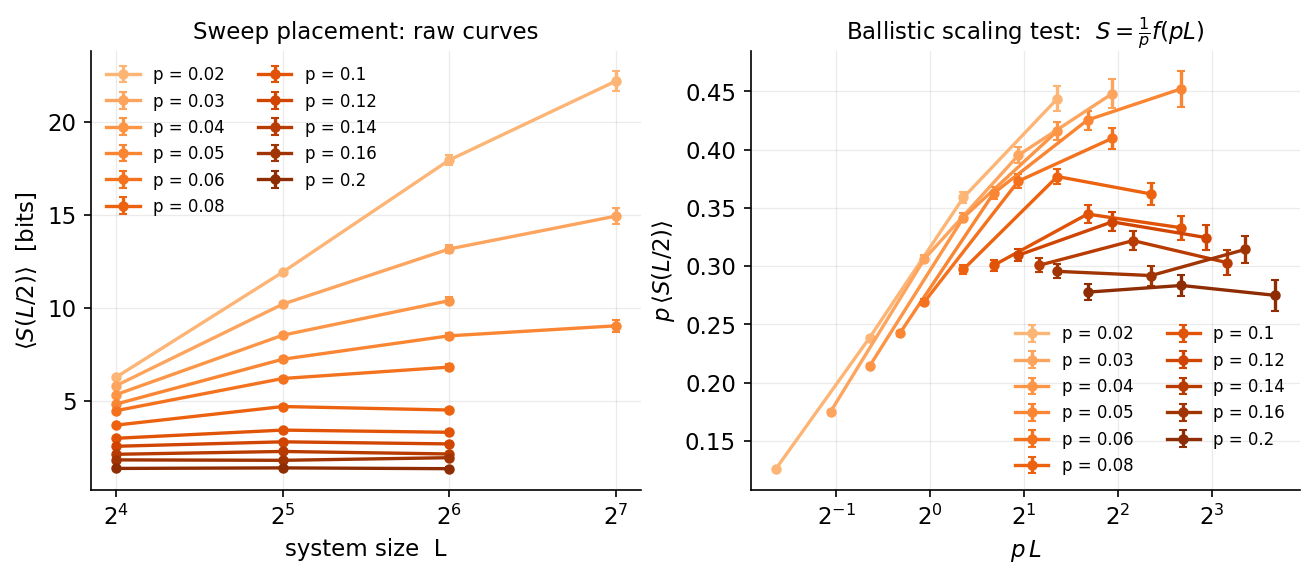
\includegraphics[width=\columnwidth]{fig6_collapse.png}
\caption{Ballistic scaling test. The rescaled entropy $p\,S$ collapses as
a function of $pL$ for $p \le 0.035$ and $L = 64$--$512$, with plateau
$f_\infty \approx 0.46$.}
\label{fig:collapse}
\end{figure}

\subsection{Baseline}
With random placement, statistically significant pairwise $\I_3$ crossings
among $L = 64$--$512$ (depth $T = 4L$, up to 2000 trajectories per point)
cluster at $p_c = 0.162 \pm 0.008$, and the largest-size pairs give
$p_c \approx 0.159$ (Fig.~\ref{fig:baseline}). Both values agree with
established results for this model~\cite{Zabalo2020}. This validates the
pipeline at the scales used below.

\subsection{The sweep}
At matched budget the sweep behaves qualitatively differently
(Fig.~\ref{fig:phaseshift}). Its $\I_3$ crossings do not converge to a
finite rate. The significant pairwise crossings recede with size: the
$(64,128)$ pair crosses at $p^\ast = 0.0085$ and the $(64,256)$ pair at
$p^\ast = 0.0056$, and both satisfy $p^\ast \sqrt{L_1 L_2} \approx 0.75$,
consistent with $p^\ast \propto 1/L$ at fixed $p^\ast L$. For the largest
pairs the curves are statistically indistinguishable over a broad window
in which $|\I_3| \lesssim 1$, and no well-defined crossing exists on our
grid, consistent with the crossing having receded below $p = 0.004$. The
half-cut entropy saturates at an $L$-independent value. At $p = 0.004$ the
$L = 512$ chain reaches $S = 106$ bits, close to the predicted ceiling of
$0.46/p = 115$ bits, and for $p \ge 0.05$ the entropy is size independent
within error bars across $L = 64$--$512$.

These observations follow from a ballistic argument, which we now state
quantitatively. The sweep front advances $pL$ sites per layer on
average, so it returns to any given cut after $1/p$ layers, independent
of $L$. In the steady state, the time $\tau$ elapsed since the front
last crossed a given cut is uniformly distributed on $[0, 1/p)$. Between
passages, the entanglement across the cut regrows at most ballistically
from the remainder $S_r$ left by the passage,
$S(\tau) \le S_r + v_E\,\tau$, where $v_E$ is the entanglement growth
velocity of the unitary dynamics. Averaging over $\tau$ gives the
steady-state bound
\begin{equation}
\langle S \rangle \;\le\; S_r + \frac{v_E}{2p},
\label{eq:ceiling}
\end{equation}
which is independent of $L$: an area law at every fixed $p > 0$, that
is, $p_c^{\rm sweep} = 0$ in the thermodynamic limit. Finite systems
interpolate between this ceiling and the volume law
$S \approx s_v L/2$ of the weakly monitored regime, where
$s_v \approx 0.46$ bits per site in our data. Equating the two scales
gives the crossover condition $s_v L/2 \sim f_\infty/p$, that is,
$pL = O(1)$: the only scale in the problem is $1/p$, and the scaling
form
\begin{equation}
S(p, L) = \frac{1}{p}\, f(pL),
\quad
f(x) \xrightarrow{\,x \to 0\,} \frac{s_v x}{2},
\quad
f(x) \xrightarrow{\,x \to \infty\,} f_\infty,
\label{eq:scaling}
\end{equation}
follows. Two independent checks confirm Eq.~\eqref{eq:scaling}. First,
it collapses the data for $p \le 0.035$ across $L = 64$--$512$
(Fig.~\ref{fig:collapse}), with $f_\infty \approx 0.46$. Second, it
predicts that finite-size $\I_3$ crossings occur at fixed $p^\ast L$,
that is, $p^\ast \propto 1/L$ rather than $p^\ast \to \mathrm{const}$ as
in Eq.~\eqref{eq:fss}; the measured crossings satisfy
$p^\ast \sqrt{L_1 L_2} \approx 0.75$, an $O(1)$ constant, as predicted.
Rates outside the $p \to 0$ scaling regime fall below the plateau, as
expected from lattice-scale corrections.

The coefficient can be checked against an independent measurement. In the
unitary circuit ($p = 0$) we measure an entanglement growth velocity
$v_E = 0.647 \pm 0.005$ bits per layer at $L = 256$. If each sweep passage
reset the entanglement at a cut to zero, the time since the last passage
would be uniform on $[0, 1/p]$ and the mean steady-state entropy would be
$v_E/(2p)$, giving $f_\infty = v_E/2 = 0.324$. The measured plateau lies
above this estimate. The direction of the discrepancy is expected: the
sweep measures sites rather than bonds, so a passage removes only part of
the entanglement across a cut, and regrowth starts from a nonzero
remainder. The scaling form itself, which is the substantive claim, does
not depend on this coefficient.

\subsection{Neither coverage nor state information is the mechanism}
\label{sec:coverage}
Table~\ref{tab:policies} isolates what makes the sweep effective, at
$L = 24$, $k = 3$ measurements per layer, and $T = 96$. The shuffled
coverage control visits every site exactly as often as the sweep but in a
spatially unstructured order, and it performs no better than random
placement. Contiguity and sequential order, not coverage, carry the
effect. The oracle-greedy policy has full access to the quantum state and
measures the sites of largest local entanglement, and it still loses to
the blind sweep by a factor of nearly three. Myopic use of complete
quantum information is worse than a fixed geometric pattern that uses no
information at all. Figure~\ref{fig:spacetime} shows the corresponding
entanglement profiles in spacetime.

\begin{table}
\caption{Final half-cut entropy at matched budget
($L = 24$, $k = 3$, $T = 96$; mean $\pm$ s.e.m.).}
\label{tab:policies}
\begin{ruledtabular}
\begin{tabular}{lcc}
Policy & Information used & $\langle S(L/2)\rangle$ [bits] \\
\hline
Random placement   & none      & $4.31 \pm 0.08$ \\
Shuffled coverage  & none      & $4.12 \pm 0.08$ \\
Oracle greedy      & quantum   & $3.56 \pm 0.09$ \\
Learned linear (CEM) & classical & $3.29 \pm 0.14$ \\
Sweep              & none      & $1.25 \pm 0.05$ \\
\end{tabular}
\end{ruledtabular}
\end{table}

\section{The information ledger}
\label{sec:ledger}

\begin{figure}
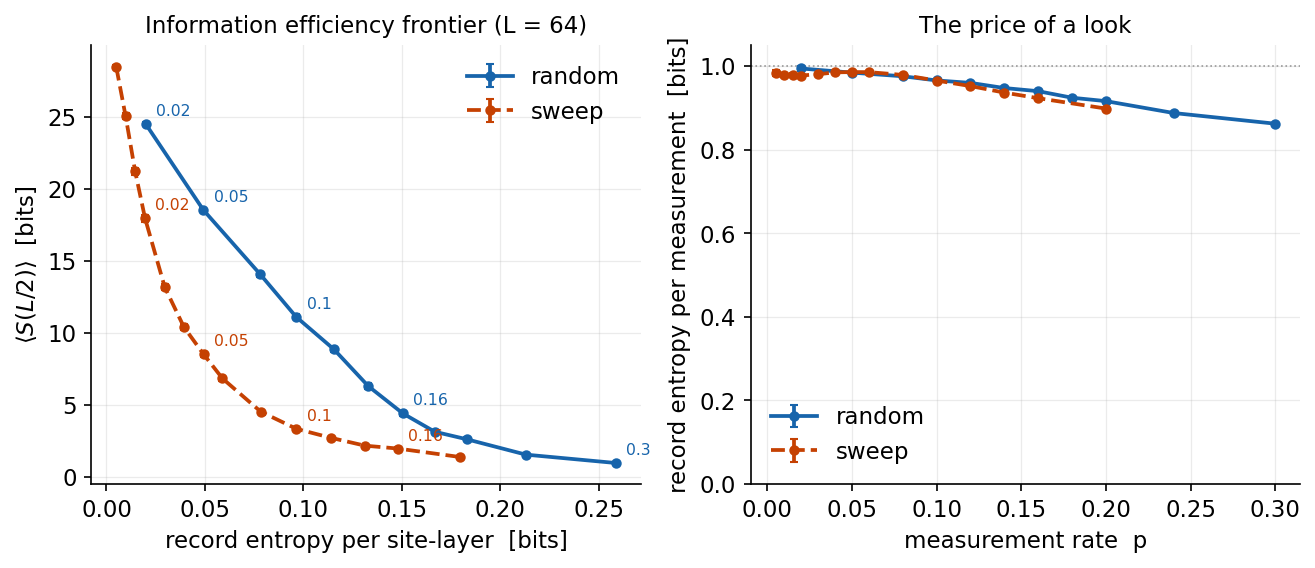
\includegraphics[width=\columnwidth]{fig7_ledger.png}
\caption{The information ledger at $L=64$. Left: the sweep dominates the
entropy-versus-record-cost frontier. Right: both placements pay
approximately one bit per measurement.}
\label{fig:ledger}
\end{figure}

The lemma of Sec.~\ref{sec:model} has a consequence that bounds what any
placement policy can achieve per recorded bit.

\emph{Proposition (one bit per bit).} In stabilizer dynamics, a
deterministic single-site measurement leaves $S_A$ unchanged for every
region $A$, and a nondeterministic one changes each $S_A$ by $0$ or
$-1$. Consequently, along any trajectory, the total entanglement removed
by measurements across any fixed cut is bounded by the record entropy:
\begin{equation}
\Delta S_{\rm meas} \;\le\; H_{\rm rec}.
\label{eq:onebit}
\end{equation}

\emph{Proof.} If the outcome is deterministic, $\pm Z_q$ is in the
stabilizer group, the projector acts as the identity on the state, and
no entropy changes. If the outcome is random, the generators can be
chosen so that exactly one anticommutes with $Z_q$, and the measurement
replaces that single generator by $\pm Z_q$. The generator matrices
before and after differ in one row, so
$\mathrm{rank}_{\mathrm{GF}(2)}(G|_A)$ in Eq.~\eqref{eq:rank} changes by
at most one, and since the two outcomes yield identical entropies,
monotonicity of entanglement under local operations forbids an increase.
Summing over the measurements of a trajectory and counting one bit per
random outcome (the lemma) gives Eq.~\eqref{eq:onebit}. \hfill$\square$

A policy's information efficiency $\eta = \Delta S_{\rm meas} / H_{\rm rec}
\le 1$ measures how much of the theoretical one-bit-per-bit budget it
converts into disentanglement.

Figure~\ref{fig:ledger} accounts for the placement protocols on this
ledger at $L = 64$. The left panel plots the steady-state entropy against
the record entropy per site-layer, parametrically in $p$. The sweep
dominates the frontier: at every record-entropy budget it reaches a lower
entanglement entropy than random placement, that is, it operates closer
to the $\eta = 1$ bound of Eq.~\eqref{eq:onebit}. The right panel
explains what the advantage is not. Both protocols pay close to one bit per measurement
across the full range of rates, because in and near the volume-law regime
almost every measured outcome is nondeterministic. The sweep does not buy
cheaper information; it allocates equally priced bits better.

Two further observations sharpen the point. First, the sweep is outcome
independent: its placement decisions use no information from the record,
so the demon needs no working memory for control, and the record can be
erased as it is written at the Landauer rate without affecting the
protocol. The entire entanglement suppression in Sec.~\ref{sec:geometry}
is therefore achieved by a demon with zero control-relevant information,
which sharpens the contrast with feedback-based adaptive circuits, where
outcome information drives the
dynamics~\cite{Iadecola2023,Sierant2023,ODea2024,Buchhold2022,Piroli2023}.
Second, the oracle-greedy policy of Sec.~\ref{sec:coverage} consumes
maximal information and still loses to the sweep, so information about the
state is neither necessary nor sufficient for effective placement at this
granularity: geometry is.

\section{Learned placement policies}
\label{sec:learned}

We ask whether placement structure can be learned rather than designed.
Policies observe only classical record features per site: time since the
site was last measured, last outcome, empirical outcome bias, neighbor
staleness, and layer parity. Actions select $k$ distinct sites per layer,
so all comparisons remain at matched budget.

We train two policy classes to minimize the final half-cut entropy. The
first is a linear scoring policy (top-$k$ over a linear function of the
site features) trained with the cross-entropy method. The second is a
translation-equivariant circular convolutional network with a recurrent
global memory, trained with proximal policy optimization (PPO); actions
are sampled without replacement through a Plackett--Luce factorization,
which gives exact log-probabilities. The recurrent state exists precisely
so that the policy class can express time-advancing patterns such as
sweeps. Training used 400 updates of 64 episodes (25{,}600 episodes) at
$L = 32$, $k = 4$, $T = 128$, with per-layer entropy-difference reward
shaping. Architecture and hyperparameters are given in
Appendix~\ref{app:learning}.

Table~\ref{tab:learned} reports matched-budget evaluations. The CEM linear
policy improves modestly on random placement and converges to a fencing
strategy: it pins measurements at a small set of fixed sites and
quarantines entanglement between them (Fig.~\ref{fig:spacetime}). Fencing
is locally sensible and globally suboptimal. The PPO policy, given a
policy class that contains moving patterns and $19\times$ more episodes,
does not improve on random placement ($5.17 \pm 0.12$ against
$5.34 \pm 0.08$), and its training curve is flat over the final 300
updates. Its stochasticity is doing the work: decoding the same policy
greedily performs worse ($6.28 \pm 0.15$) and writes fewer random bits to
the record, indicating collapse onto repeatedly measured sites, the
fencing failure mode again. The sweep outperforms every learned and
informed policy by more than a factor of two.

\begin{table}
\caption{Final half-cut entropy at matched budget
($L = 32$, $k = 4$, $T = 128$; mean $\pm$ s.e.m.).}
\label{tab:learned}
\begin{ruledtabular}
\begin{tabular}{lcc}
Policy & Information used & $\langle S(L/2)\rangle$ [bits] \\
\hline
Random placement       & none      & $5.34 \pm 0.08$ \\
Shuffled coverage      & none      & $4.95 \pm 0.09$ \\
PPO (stochastic)       & classical & $5.17 \pm 0.12$ \\
PPO (greedy decoding)  & classical & $6.28 \pm 0.15$ \\
Oracle greedy          & quantum   & $4.45 \pm 0.18$ \\
Sweep                  & none      & $2.00 \pm 0.07$ \\
\end{tabular}
\end{ruledtabular}
\end{table}

We read this as a statement about optimization geometry rather than about
expressivity. The sweep is representable in the PPO policy class: strong
weight on the staleness feature with a stable tie-breaking direction
implements it. The learning signal, however, is nearly myopic. One
measurement moved by one site changes the final entropy little, so the
reward landscape around unstructured policies is flat, while the sweep's
advantage is a property of a long temporally coherent trajectory of
placements. Local policy improvement does not assemble such trajectories
from unstructured starting points, and both of our learners instead find
the nearest attractor, fencing, which is a static approximation to
cutting. Learning where to measure is therefore hard not because good
strategies are complex but because their value is invisible to myopic
credit assignment.

\section{Discussion}
\label{sec:discussion}

Our results show that the phase diagram of monitored dynamics is a
property of the placement process, not only of the measurement rate. The
existing structured-placement literature, in which quasiperiodic
sublattices~\cite{Shkolnik2023} and quenched disorder~\cite{Zabalo2023}
modify the universality class but preserve the transition, might suggest
that placement structure is a marginal perturbation. The sweep shows the
opposite: structure that advances in time removes the volume-law phase
entirely at matched budget. The distinction between static and
time-advancing structure is therefore qualitative. A static pattern
leaves unmeasured regions where entanglement survives indefinitely; a
sweep guarantees that every site is refreshed on the $L$-independent
timescale $1/p$, and ballistic regrowth cannot outrun it.

Three implications follow. For theory, the measurement rate alone is an
incomplete control parameter, and statements about the volume-law phase
implicitly assume unstructured placement. For classical simulation, a
sweeping measurement schedule keeps monitored Clifford dynamics in a
low-entanglement regime at rates far below the random-placement
transition, which may extend to tensor-network simulability of
non-Clifford monitored systems. For experiments in which mid-circuit
measurements are slow or costly, entanglement suppression per measurement
is the relevant figure of merit, and placement geometry delivers more of
it than either coverage or state knowledge.

Several questions remain open. First, the crossover function $f$ and its
universality: whether $f$ depends only on the gate ensemble through
$v_E$, and how the sweep front's partial cutting renormalizes the plateau.
Second, dimensionality: in two dimensions a sweeping front of measured
sites is a line, and whether an analogous single-scale collapse holds is
unknown. Third, optimality: among outcome-independent placement processes
at fixed budget, whether the sweep minimizes the steady-state entropy, and
what the corresponding bound is. Fourth, learning: whether curriculum
schedules, longer-horizon credit assignment, or initialization near
sweep-like policies make the geometric optimum reachable, which bears on
the broader question of when reinforcement learning can discover
temporally coherent control strategies. Finally, the ledger beyond
stabilizer circuits: for non-Clifford monitored dynamics the record
entropy is no longer a simple count, and the tradeoff between entanglement
steered and information recorded becomes a genuine thermodynamic
optimization.

\begin{acknowledgments}
Simulations were performed in part on the HYAK computing cluster at the
University of Washington. AI-based tools were used to assist with
literature search, code development, data analysis, and manuscript
preparation; the author directed this work and verified all results.
\end{acknowledgments}

\section*{Data and code availability}
The simulation code, trained policies, and the data behind the figures
are provided upon request.

\appendix

\section{Numerical methods}
\label{app:numerics}

\emph{Circuits.} Chains of $L$ qubits with periodic boundary conditions,
$L$ divisible by 4. Brickwork layers apply independent uniformly random
two-qubit Clifford gates to even bonds on even layers and odd bonds
(including the wrap bond) on odd layers. Projective $Z$ measurements
follow each gate layer according to the placement process. All runs use
depth $T = 4L$ from the product initial state $|0\rangle^{\otimes L}$.

\emph{Entropies.} All entropies use Eq.~\eqref{eq:rank} on the canonical
stabilizer generators; $\I_3$ uses Eq.~\eqref{eq:i3} with contiguous
quarters $A, B, C, D$.

\emph{Crossings.} A sign change of
$\I_3^{(L_1)}(p) - \I_3^{(L_2)}(p)$ between grid points counts as a
crossing only if the difference exceeds twice the combined standard error
at some grid point on each side of the change. This rejects spurious
crossings deep in the area-law regime where both curves vanish within
noise. Crossing positions are obtained by linear interpolation.

\emph{Statistics.} Trajectory counts per $(L, p)$ point range from 2000
($L = 64$) to 128 ($L = 512$). Quoted uncertainties are standard errors
over trajectories; the uncertainty on $p_c$ is the spread of significant
pairwise crossings.

\emph{Velocity.} $v_E$ is the slope of the ensemble-averaged $S(L/2, t)$
at $p = 0$, $L = 256$, fit over the central 80\% of a depth-$0.6L$
window, with the uncertainty given by the spread of per-trajectory
slopes (16 trajectories).

\section{Learned policy details}
\label{app:learning}

\emph{Features.} Each site presents five classical features: time since
the site was last measured and time since either neighbor was last
measured (both normalized by $L$), the last outcome ($\pm 1$, or 0 if
never measured), the empirical fraction of $+1$ outcomes at the site, and
the layer parity.

\emph{CEM linear policy.} Scores are a linear function of the site
features plus a global mean-feature term (10 parameters); the $k$ highest
scores are measured. Training used the cross-entropy method with
population 24 to 32, elite fraction $1/4$, additive noise floor $0.05$,
and 10 to 12 iterations of 16 to 24 evaluation episodes.

\emph{PPO policy.} Two circular convolutions (kernel 3, 32 channels,
ReLU) produce per-site embeddings; their mean feeds a GRU cell (32
hidden units) whose state is broadcast back to every site; a
$1\times 1$ convolution over the concatenation yields per-site logits
$\ell_i$, and a linear head on the pooled representation yields the
value estimate. Actions are $k$ distinct sites sampled without
replacement by sequential softmax (Plackett--Luce),
\begin{equation}
\pi_\theta(a_1, \ldots, a_k \mid s)
 = \prod_{j=1}^{k}
   \frac{e^{\ell_{a_j}}}
        {\sum_{i \notin \{a_1, \ldots, a_{j-1}\}} e^{\ell_i}},
\label{eq:pl}
\end{equation}
whose log-probability is exact, as required by the PPO objective
\begin{equation}
\mathcal{L}(\theta) = \mathbb{E}_t\!\left[
 \min\!\big(r_t(\theta) \hat A_t,\;
 \mathrm{clip}(r_t(\theta), 1{-}\epsilon, 1{+}\epsilon)\, \hat A_t\big)
\right],
\label{eq:ppo}
\end{equation}
where $r_t(\theta) = \pi_\theta(a_t|s_t)/\pi_{\theta_{\rm old}}(a_t|s_t)$
and $\hat A_t$ is the generalized advantage estimate. Training: Adam
with learning rate $3\times 10^{-4}$, discount $\gamma = 0.995$, GAE
$\lambda = 0.95$, clip $\epsilon = 0.2$, entropy bonus $0.01$, value
coefficient $0.5$, 4 epochs per update, 64 episodes per update, 400
updates. The reward is the per-layer decrease of the half-cut entropy,
plus the negative final half-cut entropy at the terminal step. Reward
shaping uses quantum-side information during training only; the deployed
policy acts on classical features alone.

\bibliography{refs}

\end{document}
